%% This is an example first chapter.  You should put chapter/appendix that you
%% write into a separate file, and add a line \include{yourfilename} to
%% main.tex, where `yourfilename.tex' is the name of the chapter/appendix file.
%% You can process specific files by typing their names in at the 
%% \files=
%% prompt when you run the file main.tex through LaTeX.
\chapter{Introduction}

Modeling is a game of balance. Tractability and reasonable solution times fight against the physical realities of vast length and time scales. The assumptions one makes when formulating a model directly impact the solution methods that can be brought to bare to the problem at hand. There is almost always guaranteed trade-offs between the level of simplification of a model and the amount of time needed to solve that model.

Granular media present an interesting intermediary between the world of the discrete and continuum. While often times they are studied in contexts where continuum approximations are appropriate (i.e. geological), their behavior at much smaller length scales (a bucket of sand at the beach or flow through an hour glass) are still of great interest. However at those more everyday scales, the length scale of a single grain of sand is a relatively large proportion of the scale of the entire problem, and thus cannot be ignored. And even at the larger aforementioned geological scales, the initiation of an earthquake, for an example, still relies on individual grains of sand slipping and deforming against each other.

The great challenge, then, is to formulate a model that can capture length scale effects but still have enough simplifying assumptions to make the problem solvable with efficient methods. This however seems to fly in the face of the modeling trade-off previously discussed; it is nearly impossible to have a single model that allows for fine-scale resolution and yet ignores those small length scales to become efficiently solvable. The solution proposed in this work addresses this issue by ignoring the "single" part of the "single model" clause, and instead hybridizes two distinct models to yield the two distinct attributes desired: resolution of length scale while maintaining efficient solvability.

The work is structured as follows. The remainder of chapter 1 puts the current work in the greater academic context and discusses prior work on the modeling of granular media. Hybridization models in and out of granular media contexts are also discussed. 

Chapter 2 discusses the discrete element method used and some details of its algorithmic solution. While the level of detail presented may seem overly exhaustive, it provides important context for where the hybridization technique interfaces with the discrete element method.

Chapter 3 discusses the continuum models used. The method used to solve these models, the Material Point Method, is also discussed in detail.

Chapter 4 introduces the hybridization technique. Its goal, formulation, and solution are discussed.

Chapter 5 shows examples of the hybridization technique at work, with comparisons to the discrete and continuum model solutions, as well as to literature.

Finally chapter 6 concludes the thesis and discusses future work. 

\section{Granular Media Modeling}

The ubiquity of granular media in everyday life cannot be understated. We walk on it on trails, drive over it on roads \cite{sullivan06}, ingest it in our pharmaceuticals, and eat it in our meals. Slightly less directly, granular media is second only to water for the type of material most commonly handled in industry \cite{Richard:2005:Slow}. Despite this ubiquity however, a comprehensive model that can capture the behavior of granular media remains elusive.


\begin{figure}[htp] 
    \centering
    \subfloat[data a]{%
        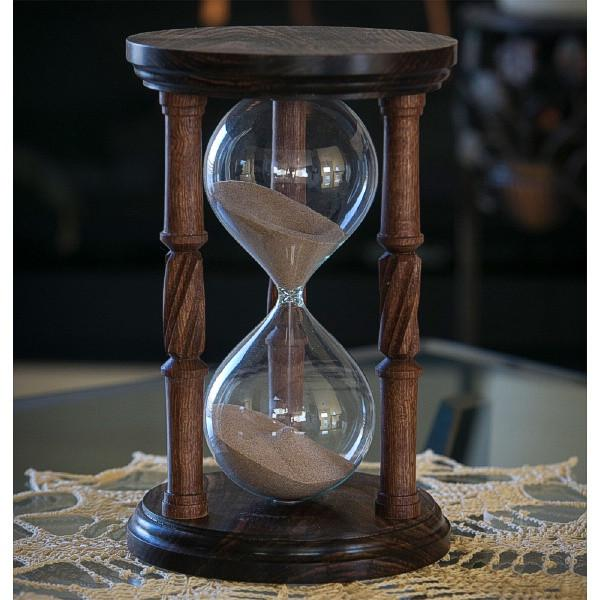
\includegraphics[width=0.4\textwidth]{figs/hourglass_whole.jpg}%
        \label{fig:a}%
        }%
    \hfill%
    \subfloat[data b]{%
        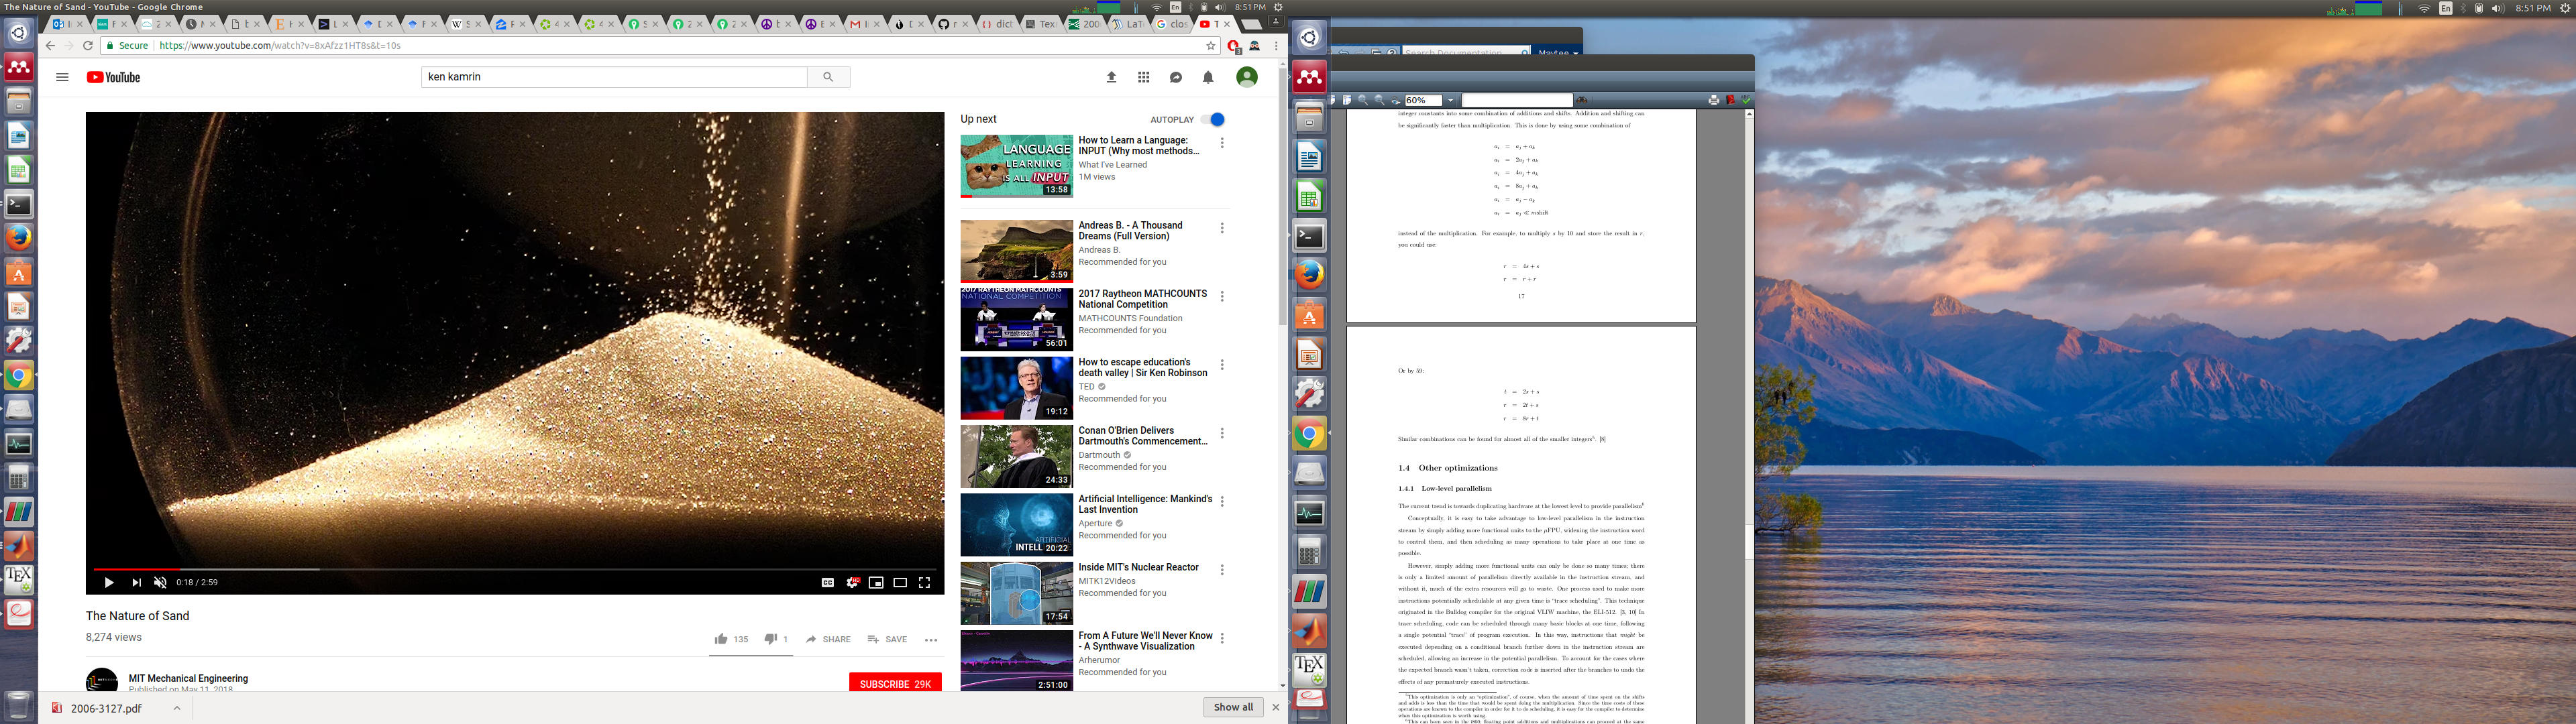
\includegraphics[width=0.4\textwidth]{figs/hourglass_closeup.png}%
        \label{fig:b}%
        }%
    \caption{Flowing hourglass displaying three distinct phases, with entire hourglass 			(a) and closeup of bottom region (b)}
    \label{hourglass}
\end{figure}

While much of the difficulty stems from the length and time scale problems mentioned before, granular media is also unique from many other materials in its ability to transition between different states. This is clearly evident in a flowing hourglass, as shown in Figure \ref{hourglass}. At the bottom of the hourglass, settled sand acts as a solid, able to support compressive stress without flowing. At the top of the static pile is a region of grains flowing over the static region, acting like a liquid. In between the top and bottom of the hourglass the grains flow much like a dilute gas, with no cohesive structure and interacting via collisions.

Different models and solution techniques are able to capture granular behavior in a given state, though of course with trade-offs in accurately capturing behavior in other states. A summary of different methods are thusly discussed. 

\subsection{Discrete Methods}



\subsection{Continuum Methods}

\subsection{Related Hybridization Work}

\subsection{Post Multiply Normalization}

When more than two multiplications are performed in a row, the intermediate
normalization of the results between multiplications can be eliminated.
This is because with each multiplication, the mantissa can become
denormalized by at most one bit.  If there are guard bits on the mantissas
to prevent bits from ``falling off'' the end during multiplications, the
normalization can be postponed until after a sequence of several
multiplies\footnote{Using unnormalized numbers for math is not a new idea; a
good example of it is the Control Data CDC 6600, designed by Seymour Cray.
\cite{thornton:cdc6600} The CDC 6600 had all of its instructions performing
unnormalized arithmetic, with a separate {\tt NORMALIZE} instruction.}.

% This is an example of how you would use tgrind to include an example
% of source code; it is commented out in this template since the code
% example file does not exist.  To use it, you need to remove the '%' on the
% beginning of the line, and insert your own information in the call.
%
%\tagrind[htbp]{code/pmn.s.tex}{Post Multiply Normalization}{opt:pmn}

As you can see, the intermediate results can be multiplied together, with no
need for intermediate normalizations due to the guard bit.  It is only at
the end of the operation that the normalization must be performed, in order
to get it into a format suitable for storing in memory\footnote{Note that
for purposed of clarity, the pipeline delays were considered to be 0, and
the branches were not delayed.}.

\subsection{Block Exponent}

In a unoptimized sequence of additions, the sequence of operations is as
follows for each pair of numbers ($m_1$,$e_1$) and ($m_2$,$e_2$).
\begin{enumerate}
  \item Compare $e_1$ and $e_2$.
  \item Shift the mantissa associated with the smaller exponent $|e_1-e_2|$
        places to the right.
  \item Add $m_1$ and $m_2$.
  \item Find the first one in the resulting mantissa.
  \item Shift the resulting mantissa so that normalized
  \item Adjust the exponent accordingly.
\end{enumerate}

Out of 6 steps, only one is the actual addition, and the rest are involved
in aligning the mantissas prior to the add, and then normalizing the result
afterward.  In the block exponent optimization, the largest mantissa is
found to start with, and all the mantissa's shifted before any additions
take place.  Once the mantissas have been shifted, the additions can take
place one after another\footnote{This requires that for n consecutive
additions, there are $\log_{2}n$ high guard bits to prevent overflow.  In
the $\mu$FPU, there are 3 guard bits, making up to 8 consecutive additions
possible.}.  An example of the Block Exponent optimization on the expression
X = A + B + C is given in figure~\ref{opt:be}.

% This is an example of how you would use tgrind to include an example
% of source code; it is commented out in this template since the code
% example file does not exist.  To use it, you need to remove the '%' on the
% beginning of the line, and insert your own information in the call.
%
%\tgrind[htbp]{code/be.s.tex}{Block Exponent}{opt:be}

\section{Integer optimizations}

As well as the floating point optimizations described above, there are
also integer optimizations that can be used in the $\mu$FPU.  In concert
with the floating point optimizations, these can provide a significant
speedup.  

\subsection{Conversion to fixed point}

Integer operations are much faster than floating point operations; if it is
possible to replace floating point operations with fixed point operations,
this would provide a significant increase in speed.

This conversion can either take place automatically or or based on a
specific request from the programmer.  To do this automatically, the
compiler must either be very smart, or play fast and loose with the accuracy
and precision of the programmer's variables.  To be ``smart'', the computer
must track the ranges of all the floating point variables through the
program, and then see if there are any potential candidates for conversion
to floating point.  This technique is discussed further in
section~\ref{range-tracking}, where it was implemented.

The other way to do this is to rely on specific hints from the programmer
that a certain value will only assume a specific range, and that only a
specific precision is desired.  This is somewhat more taxing on the
programmer, in that he has to know the ranges that his values will take at
declaration time (something normally abstracted away), but it does provide
the opportunity for fine-tuning already working code.

Potential applications of this would be simulation programs, where the
variable represents some physical quantity; the constraints of the physical
system may provide bounds on the range the variable can take.
\subsection{Small Constant Multiplications}

One other class of optimizations that can be done is to replace
multiplications by small integer constants into some combination of
additions and shifts.  Addition and shifting can be significantly faster
than multiplication.  This is done by using some combination of
\begin{eqnarray*}
a_i & = & a_j + a_k \\
a_i & = & 2a_j + a_k \\
a_i & = & 4a_j + a_k \\
a_i & = & 8a_j + a_k \\
a_i & = & a_j - a_k \\
a_i & = & a_j \ll m \mbox{shift}
\end{eqnarray*}
instead of the multiplication.  For example, to multiply $s$ by 10 and store
the result in $r$, you could use:
\begin{eqnarray*}
r & = & 4s + s\\
r & = & r + r
\end{eqnarray*}
Or by 59:
\begin{eqnarray*}
t & = & 2s + s \\
r & = & 2t + s \\
r & = & 8r + t
\end{eqnarray*}
Similar combinations can be found for almost all of the smaller
integers\footnote{This optimization is only an ``optimization'', of course,
when the amount of time spent on the shifts and adds is less than the time
that would be spent doing the multiplication.  Since the time costs of these
operations are known to the compiler in order for it to do scheduling, it is
easy for the compiler to determine when this optimization is worth using.}.
\cite{magenheimer:precision}

\section{Other optimizations}

\subsection{Low-level parallelism}

The current trend is towards duplicating hardware at the lowest level to
provide parallelism\footnote{This can been seen in the i860; floating point
additions and multiplications can proceed at the same time, and the RISC
core be moving data in and out of the floating point registers and providing
flow control at the same time the floating point units are active. \cite{byte:i860}}

Conceptually, it is easy to take advantage to low-level parallelism in the
instruction stream by simply adding more functional units to the $\mu$FPU,
widening the instruction word to control them, and then scheduling as many
operations to take place at one time as possible.

However, simply adding more functional units can only be done so many times;
there is only a limited amount of parallelism directly available in the
instruction stream, and without it, much of the extra resources will go to
waste.  One process used to make more instructions potentially schedulable
at any given time is ``trace scheduling''.  This technique originated in the
Bulldog compiler for the original VLIW machine, the ELI-512.
\cite{ellis:bulldog,colwell:vliw}  In trace scheduling, code can be
scheduled through many basic blocks at one time, following a single
potential ``trace'' of program execution.  In this way, instructions that
{\em might\/} be executed depending on a conditional branch further down in
the instruction stream are scheduled, allowing an increase in the potential
parallelism.  To account for the cases where the expected branch wasn't
taken, correction code is inserted after the branches to undo the effects of
any prematurely executed instructions.

\subsection{Pipeline optimizations}

In addition to having operations going on in parallel across functional
units, it is also typical to have several operations in various stages of
completion in each unit.  This pipelining allows the throughput of the
functional units to be increased, with no increase in latency.

There are several ways pipelined operations can be optimized.  On the
hardware side, support can be added to allow data to be recirculated back
into the beginning of the pipeline from the end, saving a trip through the
registers.  On the software side, the compiler can utilize several tricks to
try to fill up as many of the pipeline delay slots as possible, as
seendescribed by Gibbons. \cite{gib86}


